\chapter{Layered Editor Architectures}
\label{chap:layeredArchs}
{\em *** Version: \today~ ***}



\bc
* fix gesture to edit Rendering, unless gesture becomes something special
* rendering or presentation? Rendering is more clear, but editing the rendering does not make sense. (maybe just explain)

HOE HEEFT PRE HIERMEE TE MAKEN? pre geeft geen berekening, maar alleen verband, dus zelfs als level i opgeleverd door pre, dan nog is het invoer

- Numbering 0 = doc, downwards like lines on a page.
** ?Add a $lower = EDIT~levels~gesture$ condition that states the result is what we mean with the gesture?



IMPORTANT there seems to be an invariant that for a j:  i>j, all mappings are correct 
  ..           ...       
 .  .    ..   .   .   .. 
.    ....  ...     ...  .
 no it's not asymmetric. find out more about this.
 maybe it's just that a level is never presented twice without intr, and vice versa



\ec
MAYBE DO SOME NON layered stuff first? to explain what spec. will mean. more important if things like intention of edit op is added as an equation.


% intro

prev. chap. spec for layer but not edit and transform. Edit result in new lower level, initiated by gesture from user. Transform higher. In this level take all layers together and connect. At top and bottom, some extra stuff.
Next chapter, we give Haskell for the combination.


First connect everything, with direct edit ops. 
Later, support for indirect and skipping.
\fromHere  % VVVVVVVVVVVVVVVVVVVVVVVVVVVVVVVVVVVVVVVVVVVV

\section{Specifying a layered editor}

The basic component for connecting the layers is the incremental specification of a single layer, given in Section~\ref{sect:maintainingInc} of the previous chapter. The specification of a layered editor consists of a composition of several instances of the single layer specification. Before we connect the specifications, we first construct a diagram that sketches the composition process.


\subsection{Connecting layers in a diagram}
\note{Add arrow for intended gesture update?}

The lefthand side of Figure~\ref{singleToMulti} shows a simplified version of the final diagram (Figure~\ref{maintainExtraState}) from Section~\ref{sect:maintainingInc}. Except for the level updates, all internal data flow is hidden, showing only the input and output values of the level. The updates are not hidden, because some updates need to be removed for the composition.

\begin{figure}\begin{small}\begin{center}\begin{center}
\epsfig{file=pics/eps/singleToMulti.eps, width=125mm}\end{center}
\caption{A single layer vs. Layer $i$.}\label{singleToMulti} 
\end{center}\end{small}\end{figure}\note{split this figure in two figures next to each other?}

In order to compose the layer, the $H$ and $L$ subscripts are replaced by indices $i$ and $i+1$, and the functions ${\tt interpret}$ and ${\tt present}$ also get subscripts. The righthand side of Figure~\ref{singleToMulti} contains the result of the transformations. Note that the abstract functions $Edit$ and $Transform$ have been dropped because adjacent layers will now take care of their functionality.

The layer in Figure~\ref{singleToMulti} cannot be composed yet, because on interpretation and presentation, it updates both the upper level ($i$) and the lower level ($i+1$). Therefore, we drop one update in the interpration phase and one in the presentation phase. Section~\ref{sect:incrementalSpec} explained that an implementation of a mapping function may perform an update on the source level of the mapping (ie. $interpret$ may update the lower level, and $present$ may update the higher level). Hence, we drop the updates on the target level: the higher level update in the interpretation phase (upper left dotted arrow), and the lower level update in the presentation phase (lower right dotted arrow). 

The lefthand side of Figure~\ref{connectingLayers} shows a layer without the two target level updates. When several layers are composed, we get the diagram on the righthand side of the figure.

\begin{figure}\begin{small}\begin{center}\begin{center}
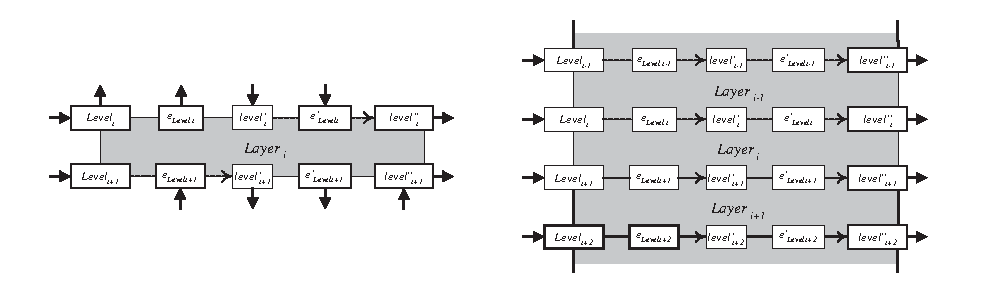
\epsfig{file=pics/eps/connectingLayers.eps, width=125mm}\end{center}
\caption{A layer with only two updates vs Composed layers}\label{connectingLayers} 
\end{center}\end{small}\end{figure}

The composition in Figure~\ref{connectingLayers}, shows what happens for internal layers that are surrounded by other layers. However on the top and the bottom of the layer composition, still some work needs to be done. At the top, edit operations coming out of the interpretation phase need to be put back into the presentation phase. And at the bottom, an edit gesture from the user must be put into the layer composition, and an updated rendering must be shown to the user. The lefthand side of Figure~\ref{topAndBottom} shows the loose ends that need to be dealt with.

\begin{figure}\begin{small}\begin{center}\begin{center}
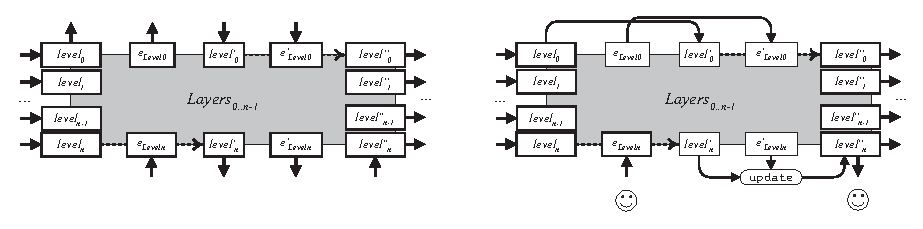
\epsfig{file=pics/eps/topAndBottom.eps, width=125mm}\end{center}
\caption{Loose ends at the top and bottom vs Dataflow at the top and bottom}\label{topAndBottom} 
\end{center}\end{small}\end{figure}

\note{gesture depends on level, not edit. Also on other levels?}

The result of the composed interpreted mappings is a document edit operation $e_{Level_0}$. Because the target update of each layer has been dropped, the operation is not performed on the document $level_0$. Rather than explicitly adding an update, we put the level and the edit operation back into the presentation part of the composed layers. This way, the document update is performed by the presentation phase of the top layer.

Similar to situation at the top, the bottom of the composition also misses an update. Therefore, we add an update at the bottom right, which applies $e'_{Level_n}$ to $level'_n$. Furthermore, the edit gesture from the user needs to be fed into the layer structure, and the updated lower level needs to be shown to the user. The righthand side of Figure~\ref{topAndBottom} shows the data flow at the top and the bottom of the composed layers.

\subsection{Specifying connected layers}

We construct of the specification of the connected layers along the same lines as the diagrams in the previous section. Recall that the data level definitions from a multiple layer perspective (see Section~\ref{sect:mappingInformation}) are:

\begin{small}\( \begin{array}{lcl}  \label{inv:incrementality}
\text{\bf type}~Level_{0}  =  Core_{Intr,0} \times Extra_{Intr,0} \times Info\idwn_{0} \\
\text{\bf type}~Level_{n}  =  Core_{Pres,n} \times Extra_{Pres,n} \times  Info\iup_{n}\\
\lefteqn{\forall j:1 \le i \le n-1:}  \\
\text{\bf type}~Level_{j} =  Core_{Pres,j} \times Extra_{Pres,j}  \times Info\iup_{j}   
                                       =  Core_{Intr,j} \times Extra_{Intr,j} \times Info\idwn_{j}
\end{array}\)\end{small}

First, we take the  final single layer specification from Section~\ref{sect:maintainingInc}, and replace the $H$ and $L$ subscripts by $i$ and $i+1$. Except for ${\tt update}$, the values and functions without an $H$ or $L$ subscript in specification~\ref{spec:incrementality} (${\tt sheet}$, ${\tt interpret}$, ${\tt present}$, and
 ${\tt reuse}$) are now specific to a certain layer and get an $i$ subscript. Because $update$ is a generic function it can be used in all layers. Finally, we drop the equations for $Edit$ and $Transform$.

\begin{small}
\refstepcounter{specification} \label{spec:compositionFirstAttempt}
\( \begin{array}{lcl}
{\tt interpret_i}  ::  Sheet_{Intr,i} \rightarrow Level_{i+1} \rightarrow Level_{i} \rightarrow  Edit_{Level_{i+1}} \rightarrow Edit_{Core_{i}\times Info\idwn_{i}} \\
{\tt present_i}  ::  Sheet_{Pres,i} \rightarrow Level_{i} \rightarrow Level_{i+1}  \rightarrow Edit_{Level_{i}} \rightarrow Edit_{Core_{i+1}\times Info\iup_{i+1}}\\
\\
\end{array}\) \\
\( \begin{array}{rcll}  
level_{i+1} 	& = & Present_{i}~level_{i}						& \text{\{Precondition\}}\\
\\
level'_{i+1} 	& = & {\tt update}~e_{Level_{i+1}}~level_{i+1}                 & \text{\{Compute intermediate lower level\}}\\
e_{Core_{i} \times Info\idwn_{i}}  & = & {\tt interpret}_{i}~sheet_{Intr,i}~level_{i+1}~level_{i}~e_{Level_{i+1}} & \text{\{Compute higher core update\}}\\
e_{Level_{i}} & = & {\tt reuse}_{Intr,i}~level_{i}~e_{Core_{i}\times Info\idwn_{i}}     & \text{\{Reuse extra state\}}\\
level'_{i} & = & {\tt update}~e_{Level_{i}}~level_{i}                 & \text{\{Compute intermediate higher level\}}\\
\\\
level'_{i} & = & Interpret_{i}~level'_{i+1}						& \text{\{Intermediate condition\}}\\
\\
level''_{i} & = & {\tt update}~e'_{Level_{i}}~level'_{i}                 & \text{\{Compute final higher level\}}\\
e'_{Core_{i+1}\times Info\iup_{i+1}}  & = & {\tt present}_{i}~sheet_{Pres,i}~level'_{i}~level'_{i+1}~e'{Level_{i}} & \text{\{Compute new lower core\}}\\
e'_{Level_{i+1}} & = & {\tt reuse}_{Pres,i}~level_{i+1}~e'_{Core_{i+1}\times Info\iup_{i+1}} & \text{\{Reuse extra state\}}\\
level''_{i+1} & = & {\tt update}~e_{Level_{i+1}}~level_{i+1}                 & \text{\{Compute final lower level\}}\\
\\
level''_{i+1} & = & Present_{i}~level''_{i}						& \text{\{Postcondition\}}\\
\end{array}\)
\end{small}
\begin{center}(Specification \thespecification: First attempt)\end{center}\vspace{1em}

\note{what to do about levels and layers subscript mismatch layers 0..n-1 levels 0..n?}

The specification does not yet define $e_n$ and $e'_0$, and similar to the diagrams of the previous section it has double updates on all levels but the document and the rendering. This is because updates for ${\tt level}$ and ${\tt level'}$ are specified on the higher level $i$ as well as the lower level $i+1$. We solve the problem in the same way as in the previous section, by dropping the updates on the target levels (\{Compute intermediate higher level\} and \{Compute final lower level\}). The updates that are left are:

\begin{small}\( \begin{array}{lcll} 
level'_{i+1} 	& = & {\tt update}~e_{Level_{i+1}}~level_{i+1}                 & \text{\{Compute intermediate lower level\}}\\
level''_{i} & = & {\tt update}~e'_{Level_{i}}~level'_{i}                 & \text{\{Compute final higher level\}}\\
\end{array}\)
\end{small}

Because of the dropped updates, there are no computations for $level'_0$ and $level''{n}$. And moreover, $e_n$ and $e'_0$ need to be defined. At the top, the document and the edit operation on it ($level_0$ and $e_0$) are put back into the computation by assigning them to $level'_0$ and $e'_0$, yielding:

\begin{small}\( \begin{array}{lcll} 
e'_{Level_{0}}  = e_{Level{0}}\\
level'_{0} =  level_{0}\\
\end{array}\)
\end{small}

At the bottom, we add a rendering update on $level'_n$ and specify that $e_n$ is the edit gesture that comes from the user. The fact that the updated rendering $level''_n$ is shown to the user is not explicitly visible in the specification.

\begin{small}\( \begin{array}{lcll} 
e_{Level_{n}}  = EditGesture ??\\
level''_{n}  =  {\tt update}~e'_{Level_{n}}~level'_{n}\\
\end{array}\)
\end{small}

If we remove the double updates and add the equations for handling the top and bottom cases, we get the final specification:

\begin{small}
\refstepcounter{specification} \label{spec:composition}
\( \begin{array}{lcl} 
\text{\bf type}~Level_{0}  =  Core_{Intr,0} \times Extra_{Intr,0} \times Info\idwn_{0} \\
\text{\bf type}~Level_{n}  =  Core_{Pres,n} \times Extra_{Pres,n} \times  Info\iup_{n}\\
\lefteqn{\forall j:1 \le i \le n-1:}  \\
\text{\bf type}~Level_{j} =  Core_{Pres,j} \times Extra_{Pres,j}  \times Info\iup_{j}   
                                       =  Core_{Intr,j} \times Extra_{Intr,j} \times Info\idwn_{j}\\
e_{Level_{n}}  = EditGesture ??\\
e'_{Level_{0}}  = e_{Level{0}}\\
level'_{0} =  level_{0}\\
level''_{n}  =  {\tt update}~e'_{Level_{n}}~level'_{n}\\
\lefteqn{\forall i:0 \le i \le n-1:}  \\
{\tt interpret_i}  ::  Sheet_{Intr,i} \rightarrow Level_{i+1} \rightarrow Level_{i} \rightarrow  Edit_{Level_{i+1}} \rightarrow Edit_{Core_{i}\times Info\idwn_{i}} \\
{\tt present_i}  ::  Sheet_{Pres,i} \rightarrow Level_{i} \rightarrow Level_{i+1}  \rightarrow Edit_{Level_{i}} \rightarrow Edit_{Core_{i+1}\times Info\iup_{i+1}}\\
\\
\end{array}\) \\
\( \begin{array}{rcll}  
level_{i+1} 	& = & Present_{i}~level_{i}						& \text{\{Precondition\}}\\
\\
level'_{i+1} 	& = & {\tt update}~e_{Level_{i+1}}~level_{i+1}                 & \text{\{Compute intermediate lower level\}}\\
e_{Core_{i} \times Info\idwn_{i}}  & = & {\tt interpret}_{i}~sheet_{Intr,i}~level_{i+1}~level_{i}~e_{Level_{i+1}} & \text{\{Compute higher core update\}}\\
e_{Level_{i}} & = & {\tt reuse}_{Intr,i}~level_{i}~e_{Core_{i}\times Info\idwn_{i}}     & \text{\{Reuse extra state\}}\\
\\\
level'_{i} & = & Interpret_{i}~level'_{i+1}						& \text{\{Intermediate condition\}}\\
\\
level''_{i} & = & {\tt update}~e'_{Level_{i}}~level'_{i}                 & \text{\{Compute final higher level\}}\\
e'_{Core_{i+1}\times Info\iup_{i+1}}  & = & {\tt present}_{i}~sheet_{Pres,i}~level'_{i}~level'_{i+1}~e'{Level_{i}} & \text{\{Compute new lower core\}}\\
e'_{Level_{i+1}} & = & {\tt reuse}_{Pres,i}~level_{i+1}~e'_{Core_{i+1}\times Info\iup_{i+1}} & \text{\{Reuse extra state\}}\\
\\
level''_{i+1} & = & Present_{i}~level''_{i}						& \text{\{Postcondition\}}\\
\end{array}\)
\end{small}
\begin{center}(Specification \thespecification: Final specification)\end{center}\vspace{1em}

\toHere     % ^^^^^^^^^^^^^^^^^^^^^^^^^^^^^^^^^^^^^

little story about what the invariant says:

Given level0..n for which Pres holds and an edit gesture, compute level''0..n so Pres holds again.

\begin{itemize}
\item level'' is level for next edit step
\item Starting the editor?
\item level for first needs to be initialized: empty vals, Present needs to hold
\item maybe first interpret is initializer, or load operation
\end{itemize}


%																
%																
%																
\section{Edit operations  on higher levels}
\begin{itemize}
\item assumed direct. But edit on rendering and interpreting is not true (ref chapter arch)
\item indirect and direct. Direct not until layout level, and sometimes on enr. or doc.
\item need to fix
\item consequences for es safety
\item lower are not just skips, but indirect edit op interpretations.
\item tricky. maybe need to point out diff between skipping and processing
\end{itemize}

\section{Skipping higher layers}
\begin{itemize}
\item ref to edit model chapter
\item kind of optimization. 
\item skipping cycles + es safety
\item with update on only lower ES, automatic skip, but then no problem with invariants
\end{itemize}

\section{Conclusions}

\begin{itemize}
\item ?
\end{itemize}




